\documentclass[pdflatex,sn-mathphys-num]{sn-jnl}

\usepackage{graphicx}%
\usepackage{multirow}%
\usepackage{amsmath,amssymb,amsfonts}%
\usepackage{amsthm}%
\usepackage{mathrsfs}%
\usepackage[title]{appendix}%
\usepackage{xcolor}%
\usepackage{textcomp}%
\usepackage{manyfoot}%
\usepackage{booktabs}%
\usepackage{algorithm}%
\usepackage{algorithmicx}%
\usepackage{algpseudocode}%
\usepackage{listings}%
\usepackage{lmodern}%
\usepackage{siunitx}
\usepackage{microtype}
\usepackage{derivative}
\usepackage[version=4]{mhchem}
\usepackage{cleveref}
\usepackage[spanish]{babel}

\renewcommand{\arraystretch}{1.2}
\sisetup{group-digits=true,
  group-separator={\,},
  separate-uncertainty
}

\raggedbottom

\begin{document}

\section*{Original English Version}

\begin{center}
  {\LARGE Silver Nanoparticles (AgNPs): Comprehensive Insights into Bio/ Synthesis,
    Key Influencing Factors, Multifaceted Applications, and Toxicity---A 2024 Update
  \par}
  \vspace{0.5cm}
  {\large Abhinav Sati, Tanvi N. Ranade, Suraj N. Mali, Haya Khader Ahmad Yasin,
  and Amit Pratap \par}
\end{center}

\vspace{0.5cm}
\noindent\textbf{Metadata}\\
Journal: ACS Omega 2025, 10, 7549--7582 \\
DOI: 10.1021/acsomega.4c11045 \\
Received: December 6, 2024 | Revised: January 29, 2025 |
Accepted: February 4, 2025 | Published: February 18, 2025 \\
Affiliations: Department of Pharmaceutical Chemistry, School of Pharmacy, D.Y.
Patil University, India; Department of Pharmaceutical
Sciences, Ajman University, UAE; Department of Oils,
Oleochemicals and Surfactants Technology, Institute of Chemical Technology,
India.
\cite{satiSilverNanoparticlesAgNPs2025}

\vspace{0.5cm}
Silver nanoparticles (AgNPs) are widely recognized for their unique optical,
electronic, and antibacterial properties, enabling their use in biosensing,
photonics, electronics, drug delivery, and antimicrobial treatments.
Green chemistry-based biological synthesis methods offer an eco-friendly
alternative to traditional chemical techniques. Among metallic
nanoparticles (NPs) and metal oxides, those derived from plant extracts exhibit
notable medicinal properties. Due to their exceptional stability
and low chemical reactivity, AgNPs are particularly well-suited for various
biological applications. AgNPs can be synthesized through chemical,
physical, or biological methods, each with distinct benefits and challenges
. Chemical and physical approaches often involve complex
purification, reactive reagents, and high energy demands, while biological
methods, though slower, provide sustainable solutions. The chosen
synthesis method strongly influences the stability, size, and purity of the
resulting NPs. This review emphasizes the importance of
selecting appropriate synthesis methods to optimize the characteristics and
functionality of silver NPs. It consolidates research spanning the
past two decades, including the most recent findings from 2024. A
comprehensive electronic search of databases such as PubMed, Scopus,
ScienceDirect, Cochrane, and Google Scholar was conducted to provide an
up-to-date overview of advances in the synthesis and applications of silver
nanoparticles.

\newpage
\selectlanguage{spanish}
\section*{Versión Traducida al Español}

\begin{center}
  {\LARGE Nanopartículas de plata (AgNPs): Perspectivas exhaustivas sobre su
    bio/síntesis, factores de influencia clave, aplicaciones multifacéticas y
  toxicidad---Una actualización de 2024 \par}
  \vspace{0.5cm}
  {\large Abhinav Sati, Tanvi N. Ranade, Suraj N. Mali, Haya Khader Ahmad Yasin,
  y Amit Pratap \par}
\end{center}

\vspace{0.5cm}
\noindent\textbf{Metadatos}\\
Revista: ACS Omega 2025, 10, 7549--7582 \\
DOI: 10.1021/acsomega.4c11045 \\
Recibido: 6 de diciembre de 2024 | Revisado: 29 de enero de 2025 |
Aceptado: 4 de febrero de 2025 | Publicado: 18 de febrero de 2025 \\
Afiliaciones: Departamento de Química Farmacéutica, Escuela de Farmacia,
Universidad D.Y. Patil, India; Departamento de Ciencias
Farmacéuticas, Universidad de Ajman, EAU; Departamento de
Aceites, Oleoquímicos y Tecnología de Tensioactivos, Instituto de Tecnología
Química, India.
\cite{satiSilverNanoparticlesAgNPs2025}

\vspace{0.5cm}
Las nanopartículas de plata (AgNPs) son ampliamente reconocidas por sus
singulares propiedades ópticas, electrónicas y antibacterianas, lo que permite
su uso en biosensores, fotónica, electrónica, administración de fármacos y
tratamientos antimicrobianos. Los métodos de síntesis biológica
basados en la química verde ofrecen una alternativa ecológica a las técnicas
químicas tradicionales. Entre las nanopartículas metálicas (NPs)
y los óxidos metálicos, aquellos derivados de extractos de plantas exhiben
propiedades medicinales notables. Debido a su excepcional
estabilidad y baja reactividad química, las AgNPs son particularmente
adecuadas para diversas aplicaciones biológicas. Las AgNPs pueden
sintetizarse mediante métodos químicos, físicos o biológicos, cada uno con
distintos beneficios y desafíos. Los enfoques químicos y físicos
a menudo implican una purificación compleja, reactivos reactivos y altas
demandas de energía, mientras que los métodos biológicos, aunque más lentos,
proporcionan soluciones sostenibles. El método de síntesis
elegido influye fuertemente en la estabilidad, el tamaño y la pureza de las
NPs resultantes. Esta revisión enfatiza la importancia de
seleccionar los métodos de síntesis adecuados para optimizar las
características y la funcionalidad de las NPs de plata. Consolida
la investigación que abarca las últimas dos décadas, incluidos los hallazgos
más recientes de 2024. Se realizó una búsqueda electrónica
exhaustiva en bases de datos como PubMed, Scopus, ScienceDirect, Cochrane y
Google Scholar para proporcionar una visión general actualizada de los avances
en la síntesis y las aplicaciones de las nanopartículas de plata.

\begin{figure}[hbt!]
  \centering
  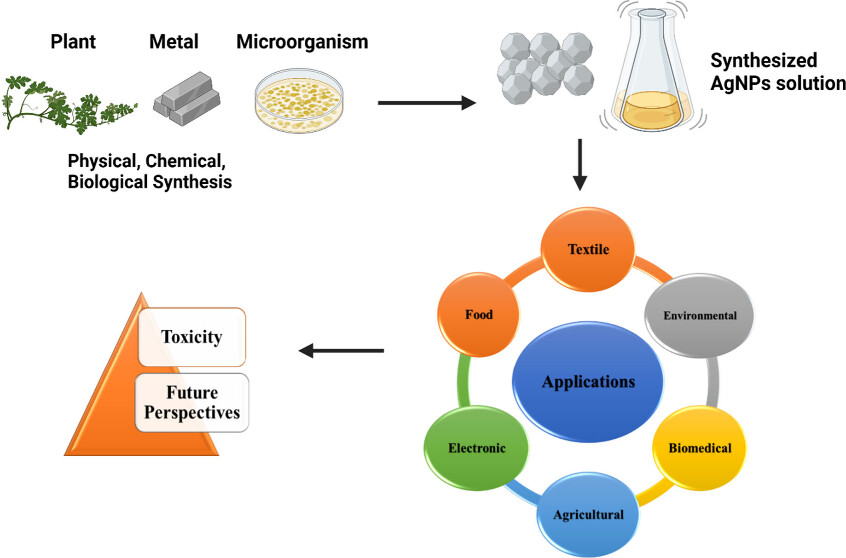
\includegraphics[width=0.8\textwidth]{./sources/graphical-abstract.jpeg}
  \caption{Resumen Gráfico}
\end{figure}

\bibliography{./silver-nano-abstract.bib}

\end{document}
